
\documentclass[acmlarge]{acmart}
%%
%% \BibTeX command to typeset BibTeX logo in the docs
\AtBeginDocument{%
  \providecommand\BibTeX{{%
    Bib\TeX}}}

%% Rights management information.  This information is sent to you
%% when you complete the rights form.  These commands have SAMPLE
%% values in them; it is your responsibility as an author to replace
%% the commands and values with those provided to you when you
%% complete the rights form.
\setcopyright{acmlicensed}
\copyrightyear{2018}
\acmYear{2018}
\acmDOI{XXXXXXX.XXXXXXX}

%%
%% These commands are for a JOURNAL article.
\acmJournal{POMACS}
\acmVolume{37}
\acmNumber{4}
\acmArticle{111}
\acmMonth{8}

%%
%% Submission ID.
%% Use this when submitting an article to a sponsored event. You'll
%% receive a unique submission ID from the organizers
%% of the event, and this ID should be used as the parameter to this command.
%%\acmSubmissionID{123-A56-BU3}

%%
%% For managing citations, it is recommended to use bibliography
%% files in BibTeX format.
%%
%% You can then either use BibTeX with the ACM-Reference-Format style,
%% or BibLaTeX with the acmnumeric or acmauthoryear sytles, that include
%% support for advanced citation of software artefact from the
%% biblatex-software package, also separately available on CTAN.
%%
%% Look at the sample-*-biblatex.tex files for templates showcasing
%% the biblatex styles.
%%

%%
%% The majority of ACM publications use numbered citations and
%% references.  The command \citestyle{authoryear} switches to the
%% "author year" style.
%%
%% If you are preparing content for an event
%% sponsored by ACM SIGGRAPH, you must use the "author year" style of
%% citations and references.
%% Uncommenting
%% the next command will enable that style.
%%\citestyle{acmauthoryear}

\usepackage{graphicx}
\usepackage{float}

%%
%% end of the preamble, start of the body of the document source.
\begin{document}

%%
%% The "title" command has an optional parameter,
%% allowing the author to define a "short title" to be used in page headers.
\title{Color Theory in VR Spaces: How Color Choice in UI Effects Educational Networking Simulations}

%%
%% The "author" command and its associated commands are used to define
%% the authors and their affiliations.
%% Of note is the shared affiliation of the first two authors, and the
%% "authornote" and "authornotemark" commands
%% used to denote shared contribution to the research.
\author{Quintin Pavilonis}
\email{quinpav@colostate.edu}
\affiliation{%
  \institution{Colorado State University}
  \city{Fort Collins}
  \state{Colorado}
  \country{USA}
}

%%
%% By default, the full list of authors will be used in the page
%% headers. Often, this list is too long, and will overlap
%% other information printed in the page headers. This command allows
%% the author to define a more concise list
%% of authors' names for this purpose.
\renewcommand{\shortauthors}{Pavilonis}

%%
%% The code below is generated by the tool at http://dl.acm.org/ccs.cfm.
%% Please copy and paste the code instead of the example below.
%%
\begin{CCSXML}
  <ccs2012>
     <concept>
         <concept_id>10003120.10003121.10003125.10010873</concept_id>
         <concept_desc>Human-centered computing~Pointing devices</concept_desc>
         <concept_significance>500</concept_significance>
         </concept>
     <concept>
         <concept_id>10003120.10003121.10003122.10003334</concept_id>
         <concept_desc>Human-centered computing~User studies</concept_desc>
         <concept_significance>300</concept_significance>
         </concept>
     <concept>
         <concept_id>10003120.10003121.10003122.10010855</concept_id>
         <concept_desc>Human-centered computing~Heuristic evaluations</concept_desc>
         <concept_significance>300</concept_significance>
         </concept>
     <concept>\begin{CCSXML}
      <ccs2012>
         <concept>
             <concept_id>10003120.10003121.10003124.10010866</concept_id>
             <concept_desc>Human-centered computing~Virtual reality</concept_desc>
             <concept_significance>500</concept_significance>
             </concept>
         <concept>
             <concept_id>10003120.10003121.10003122.10003334</concept_id>
             <concept_desc>Human-centered computing~User studies</concept_desc>
             <concept_significance>300</concept_significance>
             </concept>
         <concept>
             <concept_id>10003120.10003121.10003122.10010855</concept_id>
             <concept_desc>Human-centered computing~Heuristic evaluations</concept_desc>
             <concept_significance>300</concept_significance>
             </concept>
         <concept>
             <concept_id>10003120.10003121.10003122.10010854</concept_id>
             <concept_desc>Human-centered computing~Usability testing</concept_desc>
             <concept_significance>300</concept_significance>
             </concept>
         <concept>
             <concept_id>10003120.10003121.10003125.10010873</concept_id>
             <concept_desc>Human-centered computing~Pointing devices</concept_desc>
             <concept_significance>500</concept_significance>
             </concept>
         <concept>
             <concept_id>10003120.10003121.10003126</concept_id>
             <concept_desc>Human-centered computing~HCI theory, concepts and models</concept_desc>
             <concept_significance>500</concept_significance>
             </concept>
       </ccs2012>
      \end{CCSXML}
      
      \ccsdesc[500]{Human-centered computing~Virtual reality}
      \ccsdesc[300]{Human-centered computing~User studies}
      \ccsdesc[300]{Human-centered computing~Heuristic evaluations}
      \ccsdesc[300]{Human-centered computing~Usability testing}
      \ccsdesc[500]{Human-centered computingy~Pointing devices}
      \ccsdesc[500]{Human-centered computing~HCI theory, concepts and models}
         <concept_id>10003120.10003121.10003122.10010854</concept_id>
         <concept_desc>Human-centered computing~Usability testing</concept_desc>
         <concept_significance>300</concept_significance>
         </concept>
     <concept>
         <concept_id>10003120.10003121.10003124.10010866</concept_id>
         <concept_desc>Human-centered computing~Virtual reality</concept_desc>
         <concept_significance>500</concept_significance>
         </concept>
     <concept>
         <concept_id>10003120.10003121.10003126</concept_id>
         <concept_desc>Human-centered computing~HCI theory, concepts and models</concept_desc>
         <concept_significance>500</concept_significance>
         </concept>
   </ccs2012>
\end{CCSXML}
  
  \ccsdesc[500]{Human-centered computing~Pointing devices}
  \ccsdesc[300]{Human-centered computing~User studies}
  \ccsdesc[300]{Human-centered computing~Heuristic evaluations}
  \ccsdesc[300]{Human-centered computing~Usability testing}
  \ccsdesc[500]{Human-centered computing~Virtual reality}
  \ccsdesc[500]{Human-centered computing~HCI theory, concepts and models}



%%
%% Keywords. The author(s) should pick words that accurately describe
%% the work being presented. Separate the keywords with commas.
\keywords{Virtual Reality, VR, User Interface, UI, Networking, Human-Computer Interation, HCI}

\received{20 February 2007}
\received[revised]{12 March 2009}
\received[accepted]{5 June 2009}

%%
%% This command processes the author and affiliation and title
%% information and builds the first part of the formatted document.
\maketitle

\section{Introduction}
Accessibility has been a large focus in tech and extended reality is no different. Ensuring that users
with as wide a range of ability as possible to participate in the same digital landscape as any other. There has been emerging technology and research from
understanding and creating better user interfaces (UI) to allow ease of use to creating and adapting new hardware and input devices to accommodate more 
users with physical disabilities. These accessibility choices to consider may range from physical design of a device with the interface to the placement of menus
and icons to the very colors chosen to represent and convey information.

UI design has been intertwined with concepts such as color theory to optimize interface functionality for target users. This is due to not only to color
choice having an effect on the usability of the interface itself, but also an effect on the user's mental cognition. This concept includes how color choices might effect
how a person is able to find what they need within an interface and process how to use what they find (buttons, menus, icons). In a study on electronic note taking, it is mentioned
that color choice can even effect the emotional status of a user, "The utilization of warm colors such as red or orange has the potential to evoke feelings of excitement
or urgency, while cool colors like blue or green have the capacity to create a sense of calmness or trustworthiness." \cite{huang2024enhancing}

A gap in some technological accessibility research exists however, this research is often focused on usability and may
push other factors such a educational value factors to the wayside. Recent studies have suggested that VR may play an important and beneficial role in
the future of education, as stated here, "The results of the reviewed studies in their work show that learners who used an immersive HMD were more engaged,
spent more time on the learning tasks, and acquired better cognitive, psychomotor, and affective skills. However, this study also identifies many factors
that can be reinforcers or barriers to immersion and presence." \cite{radianti2020} which then goes on to mention factors such as color and graphics quality
having effect on learning. Further research into the fields of user accessibility and color theory may be needed to study the effects of UI color choice on user ability
to learn new information and could assists in better interfaces from simple websites to complex VR programs.

This research study has been designed to address a specific case of color in UI and their
effect on a user's ability to complete tasks based on how well they might learn them. This will specifically test how the different color icons and "wire"
connections that the user makes while learning simple networking based lessons and completing tasks based on these short lessons. A small variety of preset
and specifically chosen color palettes will be the variable that is tested for effect on user completion rate, error rate, and completion time over three short 
tests.

The following sections will cover the corresponding literature and research related to this study, the methodology designed for this study, the results, and analysis of the results.


\section{Related Work}

\subsection{Color Theory and UI Design}
The effects of color in user interface is not new and been slimming down the color choices made in interfaces of all kinds since early widespread use of computers and 
tech with interaction by lay persons. This is evident in the lack of high contrast and distracting design choices in most modern interfaces such as websites and cell phone applications.
The switch from the anything-goes-approach of design in the late 1990s to calmer and more uniform choices was a natural progression in that early technology often focuses on function rather
than form. 

The current choice to make text simple to read and not high-contrast colors was simply due to ease of use which was catalyzed by early 2000s internet shopping. The easier it is for
customer to understand a purchase and the process of the purchase, the more likely it is to complete a sell. This idea also works in simple use of technology and color choice can
alter the intended effect of an interface, as stated in a conference paper by Guoying Wen, "The main goal of UI interface color design is to express color design more perfectly with the spirit and function of mobile Internet 
application, so as to arouse users' resonance, grasp users' psychology, and gain users' recognition and understanding." \cite{wen2021color}

\subsection{Educational Application of VR}
VR in educational settings is a newer field of research but already is showing a possible benefit to learning. In a study from  The University of Northhampton in the U.K.,
it is stated "Most students also noted that an equipment like the VR headset used in the experiment can genuinely improve concentration on the topic covered in class especially in a distracting environment
(e.g., social media updates on smartphones or interruptions from other students)" \cite{slavova2018comparative} This study also mentions that the VR itself 
needs to be considered properly as "VR can potentially improve the understanding of a concept or visual information attributed to improved distraction-free engagement. However, students are less likely 
to recall or recognize specific details due to the additional cognitive load in VR." \cite{slavova2018comparative} which leads precedence to this papers research topic in color theory
in educational environments using VR.

\subsection{UI in VR}
The study of UI in virtual environments has been a mainstay subject as it represents the largest aspect of the environment communiticating information to the user.
Whether it be through simple menus similar to traditional digital environments (desktops, mobile phones), or fully encompasing environments found in video games with immersive, dynamic UIs,
the size, color, placement, shape, opacity, movement, or any other dynamic effect that an interface might have will eventually effect its overall usability. Though it is equally important to consider what not to do, especially in contained environments such as this paper's topic of color effect on VR educational environments. As mentioned in chapter 4 "Building UI in VR" in the book Google Daydream VR Cookbook: Building Games and Apps with Google Daydream, Unity, First Edition" by Same Keene "Even with the multitude of possibilities in VR, it turns out that the easiest way to consume basic information is the same way we do in the real world: on flat rectangular screens and often in text format." \cite{keene2018building} which seems almosts a paradox with the amount of possibilities within extended reality spaces, but is important to note in design nonetheless.


\subsection{Color and Learning}
Color choice has an effect on many aspects of a persons cognitive function and learning is one of them. The color of a room a person is in, the hue of the lights in the room, the color of the font on a test they are taking, can have minute effects on a persons ability to learn and then take a test on the subject matter. Whether this be a drastric example such as unreadable font choice, or the more nuanced examples previously mentioned, color choices are worth considering. In a joint study on effects on eduction in color palette choices in PowerPoints slides by 
Tianjin Normal University (Tianjin, China) and University of North Texas (Denton, USA), it is suggested that groups of colors can have positive and negative effects. "The experiment results indicate that the PPT presentation in warm colors significantly enhanced learners' transfer of knowledge of Calligraphy, and its transfer scores are marginally positively correlated with positive emotions." \cite{yang2021effect}


\section{Methodology}
\subsection{Baseline Data Collection}
This study has been conducted using two human participants that served as the range that simulated users "performed" the tests in. The baseline level of users experienced with the educational topic of networking was created using the range of user ability with error rate and completion times considered. One experienced user with networking experience and certifications served as the high end of user range and one "typical" user with only home modem setup as experience as lower end of user ability range. This ensured that all simulated profile's performances fit within realistic data ranges set by human users to give most realistic results with simulated participants. Baseline test is  the industry standard color palette (orange, green, purple, and red). All participants took part in same three test trial run using same interface placement, size, and font.

\subsection{Simulated User Profiles}
Simulated users based off the two human trials were used for this study. A group of 120 simulated participants in total were based off baseline data and subgroups of thirty were used for each color palette resulting in four groups.
Python was used to create data randomly within bounds set by baseline human trial data, and also to add noise. These data factors were completion time, error total, and 

\subsection{Simulation Runs}
Each simulated user has been "tested" using a custom python script to generate data points within the baseline scores set by human trials. Each of the four subgroups took the same three tests, with only difference being the color palette the user could choose from. Thirty users in each group were tested per color palette and the differences inside of and outside of groups was recorded. Group A had the standard industry colors (orange, green purple, red) that may be seen in professional networking environments, Group B had standard educational colors (red, green, blue, yellow), Group C had a bright, distracting palette and finally Group D had a version for colorblind friendliness. This allowed for realistic color palettes to be tested where no palette stood out too much as overly distracting.

\subsection{Tests}
All participants took three standardized tests in which they display basic networking functions after a brief rundown on simple connections involving routers, switches, and common devices such as personal computers and mobile phones. These three tests increase in difficulty by having the participant make the correct wire connections to achieve a preset goal. The first test involves connecting a home style setup with router and devices. The second test involves the use of a switch in addition to the router and devices from previous test to simulate a small office or small home network. The third test will build on second test and include second switch and more devices to simulate multi network office environment. The brief introductory phase will involve short description of router and switch and their roles in different networking environments. The only difference between tests were the different color palettes used for the simulated wire connections based on participant grouping. These tests are designed to allow for a basic introduction to simple and common networking setups as not to overwhelm the participants will complex networking information. This was important to keep the focus of the study on the effects of how color affects participant performance in these tests.

\subsection{Statistical Analysis}
Standard ANOVA testing was done on the results to asses levels of variance found within and between groups. Groups of thirty were used to result in medium effect size with power of 80\%.

\section{Results}

\subsection{Disclaimer}
It is important to note that nearly all of the data used in analysis was simulated and results should be treated as a proof of concept for this prototype, and are not to be used in research. Two human participants were tested to establish realistic bounds for data to be simulated, for which 120 users were simulated from these results.

\subsection{Task Completion Time}
Results show that the distracting palette had the lowest mean completion time overall for all three tests at 93.1 seconds. The lowest completion time for any single test was for test 1, using the distracting palette at 64.86 seconds as seen in figure 1 below. This seems a contradiction of the name and purpose of the distracting palette in the intent to be a visually harder to look set of colors. The completion time increasing coincided with the raise in difficulty for each test. The standard deviations for all palettes are large which suggests a significant amount of variability in user ability.

\begin{figure} [H]
  \centering
  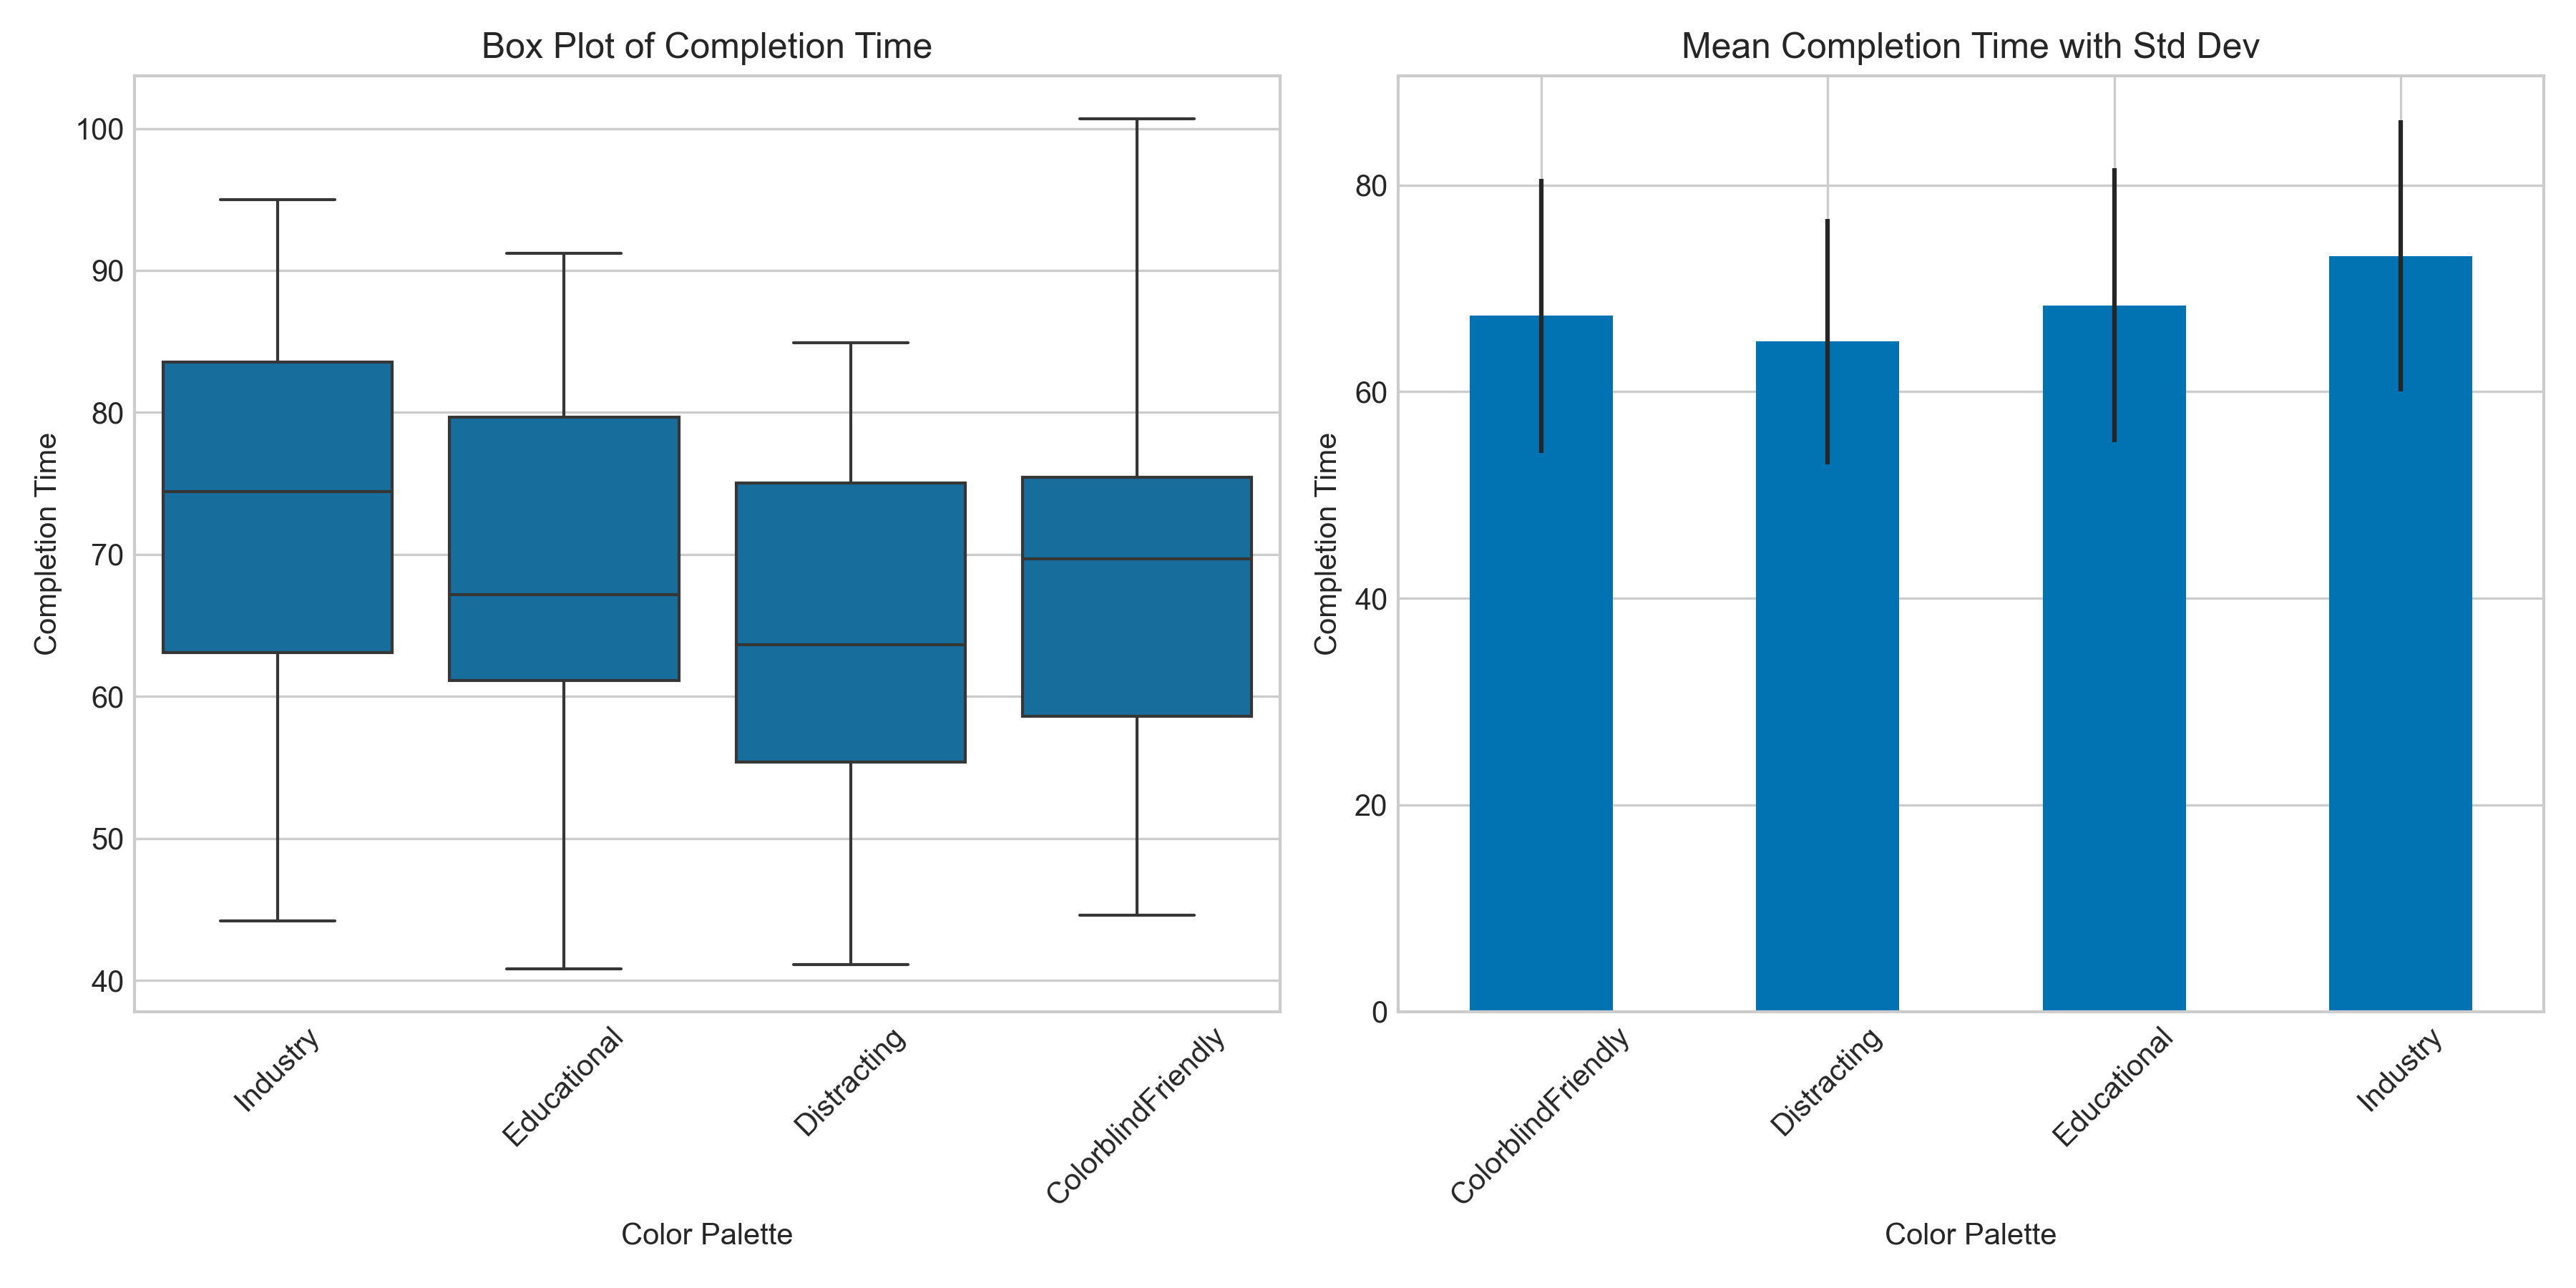
\includegraphics[width=0.8\textwidth]{completion_time_test1_analysis_20250504_061112.png}
  \caption{Comparison of completion times across different color palettes for Test 1. The box plot (left) shows the distribution of completion times, while the bar chart (right) displays mean completion times with standard deviation.}
  \label{fig:completion-time-test1}
\end{figure}

\subsection{Error Rate}
Error rates are recorded when user makes an incorrect connection by using the wrong color. The colorblind friendly palette showed lowest overall mean error of 3.49 errors per all three tests. The industry standard color palette showed the worst results at an mean of 3.79 errors, including test 3 which had a high of 8 errors, which is similar to all test 3 results.

\begin{figure} [H]
  \centering
  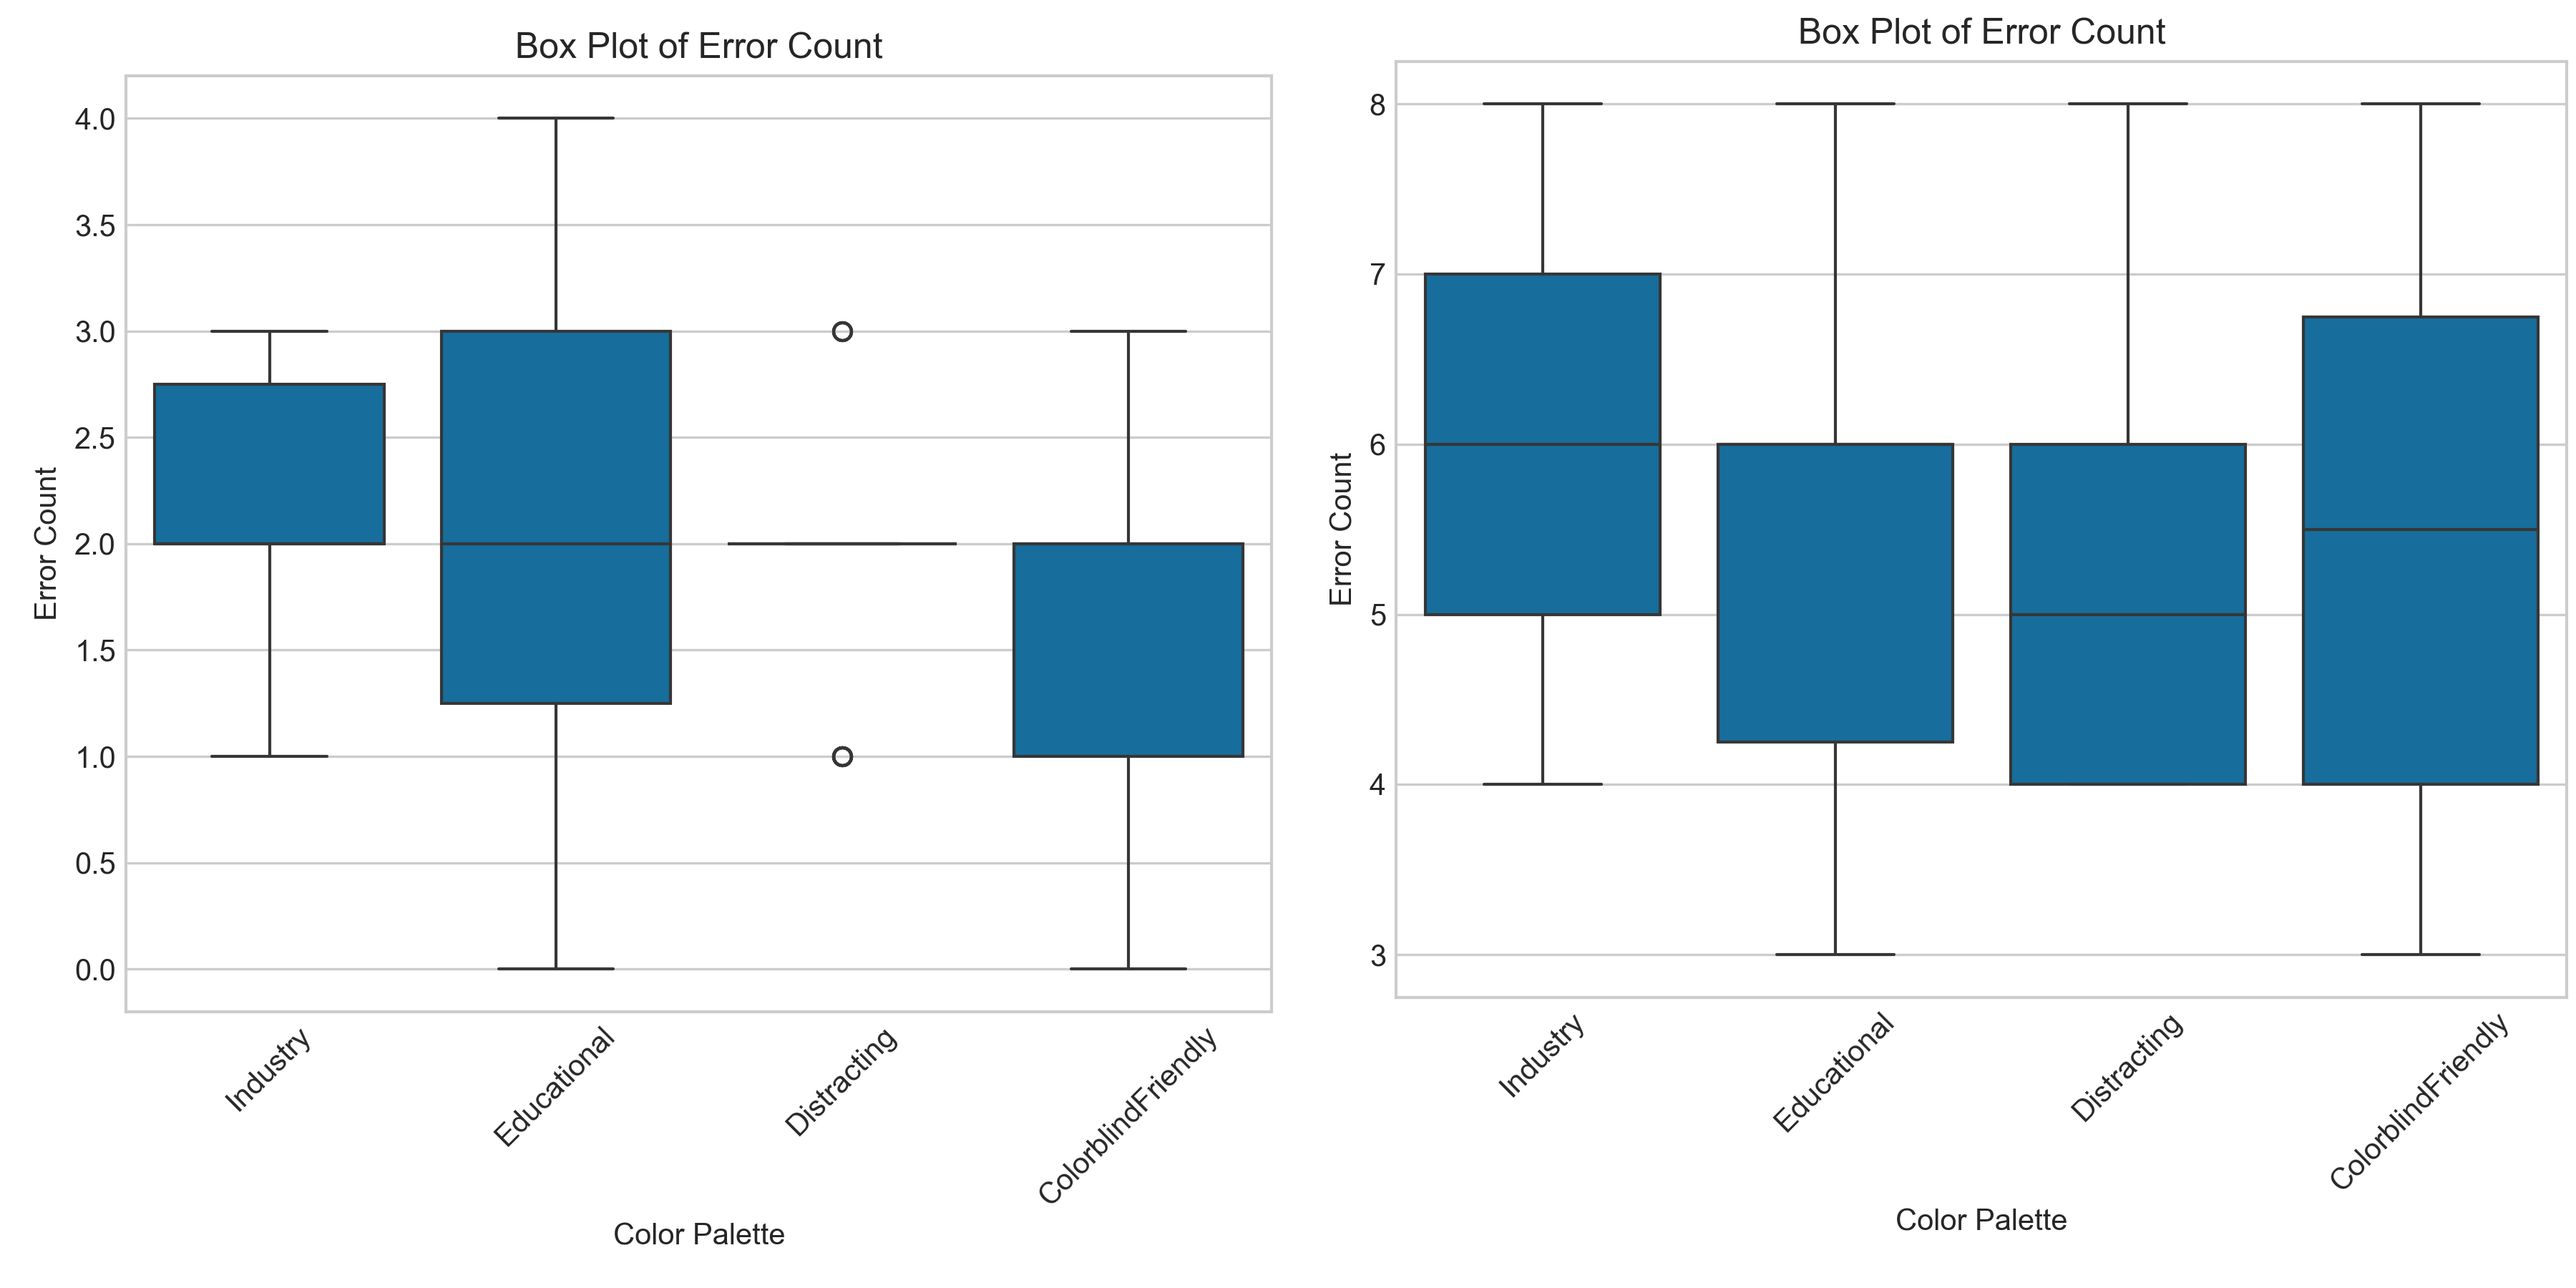
\includegraphics[width=0.8\textwidth]{errorcounttest1and3.png}
  \caption{Comparison of error counts across different color palettes for Test 1 (left) to Test 3 (right), showing an increase of errors made as tests increase in difficuly.}
  \label{fig:errorcounttest1and3}
\end{figure}

\subsection{Task Success Rate}
Task success was calculated to be percentage rate of connections that were correctly implemented and the distracting color palette in the lead with 84\% and the industry standard palette at bottom with 80\%. This shows a small but evident increase in using distracting color palettes though the spread of 4\% over the four different palettes is not large. 

\subsection{Color Palette Comparison}
Overall the distracting color palette has shown signs having the most positive effect on user performance and the industry standard palette showed the most negative effects. A p-value of < 0.05 was used in one way ANOVA analysis to determine statistical significance in which completion time for test 2 and 3 had f-values of 2.75 and 3.08 respectively. These f-values in ANOVA show how much variation exists between color palette groups compared to variation within each group and higher values (around 3 and higher) suggest that color choice might have a measurable effect as opposed to lower values found elsewhere in the data. In a real study this would indicate the possibility that color palette choice could have a measurable effect on user performance of network based, education VR tools.

With the simulated data being the largest portion of the data collected however, this clear statistical benefit of not only color choice, but specifically the distracting color palette, can be attributed to the human user data. One of the two human participants self reported in a follow up questionnaire that they were an expert in networking knowledge, making the palette they used have the highest scores by way of being assigned to that palette. 

\section{Discussion}
\subsection{Interpreting the Results}
Within the simluated data analysis, completion time was found to have the most significant f-values of 3 and higher while error count and success rate hovered around 1.5. P-values of .045 and .030 were found for completion time within test 2 and 3 showing the change in color palette used had the largest effect on the harder tests.

In a real study using non-simulated data, the results would show a statistical significance in using the distracting color palette which would go against a natural hypothesis of assuming that distracting colors would make performance worse. However due to the necessary simulation of data, and considering that the basis of the study involves eyesight which cannot be simply replicated with scripts, these factors invalidate these findings. 

\subsection{Limitations of Study}
There were several limitations imposed on the study by natural bounds. The first and most important of note is that user data was simulated. Baseline data was established using human participants to create a realistic range for simulated data to fall within and despite this, data that is fully simulated cannot capture all variables and unmeasured effects of human computer interaction (HCI) within a VR environment.

The datasets were formulated as being two separate concepts, the first being a set that represents performance on the network test itself and data points related such as completion time and error rate. The second being HCI focused data points such as time to move controller from place to place and time spent gazing at specific places in VR environment. Simulated data in this sense will not be able to used to establish further data points or theories.

The human data sets used as ranges for simulated data are significantly limited as well with a sample size of  (n=2) presenting another level of generalization in the end results. This limitation has been acknowledged to show lack of representation of the diversity found in ability, prior knowledge, and learning speed found in human populations.

Another limitation is placed by the focus of the study being on color in educational environment specifically within in simple IT networking. Results from a study that may be set similarly or completely the same but with non-simulated data may find that results are very specific and may not be representative of performances in other educational contexts, especially those where color make take a different role than like in networking cable colors.

The limitations on this study suggest that current data analysis and methodology should only be viewed as exploratory and as a study that sets up a framework for further research into color usage in educational VR environments.

\subsection{Applications}
Although the previously mentioned limitations exist, this studies structure and methodology may be practical in several applications, specifically within VR educational environments but potentially with some of the abstract setup as well.

The mix of simulated data based on human data used as ranges provide a template for smaller and resource limited teams to develop preliminary designs and prototype before committing to larger studies. This is a necessary trade of accessibility to create studies and fully valid data.

For the specific VR program developed in this study, it may possibly used a template for further color related studies as the program was built with modification of elements such as color palette and test requirements being central.

\section{Conclusion}
\subsection{Summary}
This study was created to research the effects of color choice in UI and how those color choices can change performance within educational testing environments. By testing four distinct color schemes in the form of industry standard, educational standard, colorblind friendly, and a distracting palette, this was attempted to find any potential influence on user performance through input tracking.

The methodology was limited in terms of baseline data by way of small human sample size and then simulated data based off of those human created data values. Additionally, the very basis of the study being centered on an aspect of vision, simulated data may not represent a wide range of real human ability within a VR environment.
Even in acknowledging the limits of the study by way of simulated data, the basis of the study establishes some groundwork in study of color theory and effects of use in UI in VR environments.

\subsection{Recommendations for Future Studies}
Either removing simulated data entirely, or increasing the human participants amount to create a more accurate baseline of data would improve data output validity significantly. The concept of the study being on effects of color choice in UI inherently relies on visual ability and this would be fully amended by using human participants instead. This would be the single largest change from this first iteration, to produce intended data output.

Increasing data tracking data-points would also expand the potential for statical significance to show in how performance is effected when different color palettes are used. Expanding on the human-computer interface related data points specifically would enhance the study value within an extended reality educational environment. 

The modularity of the testing setup allows for further color study in other fields as well. By simply changing the test prompts and icons, this study can be fitted to many other educational schemes such as chemistry, computer science, etc.

Lastly, additional multi modal features could be implemented and tracked such as more haptic feedback, audio cues, and gaze based functionality. This would allow for study into optimal modal combinations within color based studies as well.



%%
%% The next two lines define the bibliography style to be used, and
%% the bibliography file.


\bibliographystyle{ACM-Reference-Format}
\bibliography{references}

\end{document}
\endinput
%%
%% End of file `sample-acmlarge.tex'.
